
\chapter[Introduction]{Introduction}
\section{Introduction}

The lymphatic system plays an important role in the human body. Not only it is responsible for fat absorption but also for fluid balance and immunological defense. The lymphatic system is part of the circulatory system, like the blood system. The blood is composed of blood cells and plasma, which contains proteins and carries the white cells.  The plasma goes through the capillary vessels in order to reach all the human body cells therefore all cells bath in this filtered blood called lymph.  \\

This lymph has to be cleaned and recirculated, which is why the lymphatic system is used for. It takes back the lymph, makes it circulate through the human body and then returns it to the blood. In addition, the lymphatic system is composed of lymph nodes, which filter the lymph and create lymphocytes to combat invaders and protect the body. \\

As opposed to the blood circulatory system, the lymphatic system does not have a pump to make the lymph circulate; it uses muscles and breathing motion to pump the lymph through the body. \\

The study of the lymphatic system is important for cancer diagnoses and treatments. Indeed, metastasis can circulate quickly in the lymphatic system and spread the tumor cells to other parts of the body. In addition, tissue swelling called lymphedema can occur after cancer surgery, it is especially the case after breast cancer surgeries \cite{marshall_near-infrared_2010}. In order to treat the lymphedema, massage can be applied to drain the lymph fluid through the patient body and increase the lymph circulation. \\

The lymphatic system has a complex structure and varies greatly among individuals. Therefore, visualizing it correctly is a tremendous task, which requires the use of methods able to deliver accurate structural information.  The lymphatic system structure can be seen in Figure~\ref{fig:The lymphatic system} \cite{lymphatic}.

\begin{figure}[h]
\caption{The lymphatic system}
\centering
    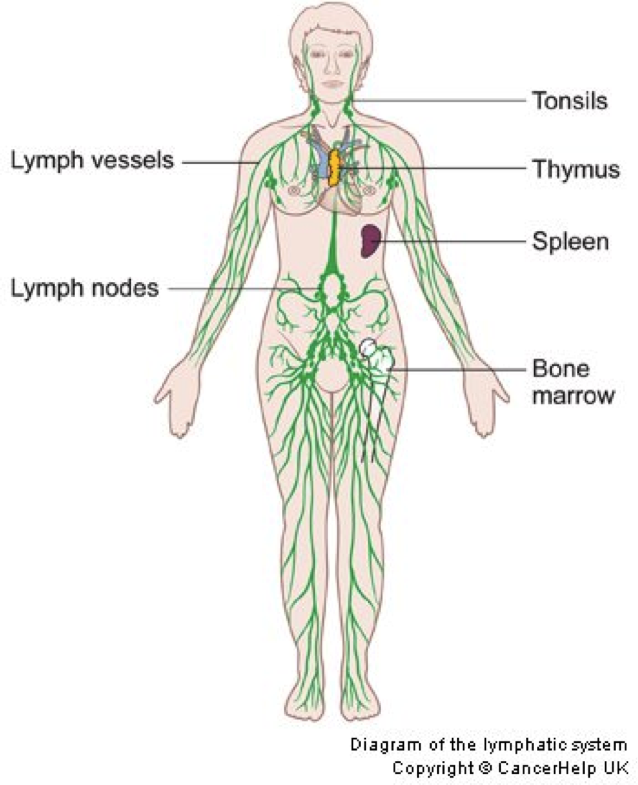
\includegraphics[width=0.7\textwidth]{images/LymphaticSystem.png}
\label{fig:The lymphatic system}
\end{figure}


According to \cite{marshall_near-infrared_2010}  "The lack of imaging to obtain structural or functional information currently limits our understanding of the role of lymphatics in disease and impedes the development of therapeutic interventions" therefore this paper introduces a novel imaging method for the lymphatic system, using infrared lights coupled with a 3D camera.

\section{Purpose}

The purpose of this project is to develop a 3D cartography tool to visualize the lymphatic system of an individual. In order to do that, a green dye called indocyanine green is injected into patients' lymphatic system. This dye has the property to be fluorescent after being exited by infrared lights therefore depth information can be acquired by using infrared cameras. However, the 3D structure only is not helpful because semantics has to be given to that 3D model, i.e. a mapping has to be applied between the lymphatic system's 3D model and the part of the human body corresponding to that 3D model (see Figure~\ref{fig:mapping1} and Figure~\ref{fig:mapping2} \cite{gianluca}). 

\begin{figure}[h]
\caption{Mapping of the lymphatic model with the corresponding body part}
\centering
    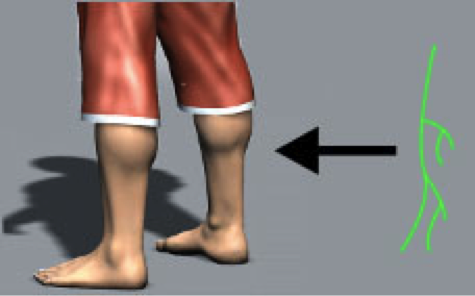
\includegraphics[width=0.7\textwidth]{images/mapping1.png}
\label{fig:mapping1}
\end{figure}

\begin{figure}[h]
\caption{Mapping done}
\centering
    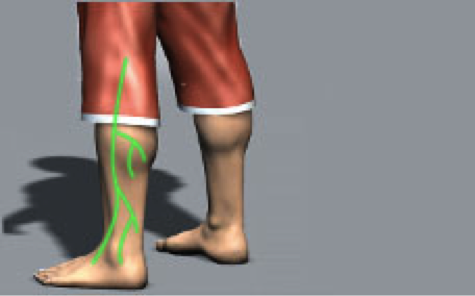
\includegraphics[width=0.7\textwidth]{images/mapping2.png}
\label{fig:mapping2}
\end{figure}

In order to do that, a 3D model of the human body is acquired through a Microsoft Kinect camera. Given an accurate 3D model of a patient and his lymphatic system, the mapping can be easily done and physicists and physiotherapists can therefore operate more easily on the patients (see Section~\ref{sec: ICG Applications}). \\

Furthermore, because cameras do not have a wide field of vision, image fusion and camera pose estimation have to be used. Image fusion consists of combining multiple images into one while camera pose estimation consists of translating the camera coordinate system into a world coordinate system. That is, determining the camera pose inside a world coordinates system. \\

This Master Thesis consists of creating a proof of concept for a novel 3D imaging acquisition system. In the first time, a basic Kinect camera coupled with a normal webcam will be used to acquire a 3D representation of an object. The Kinect will acquire a 3D surface of the object while the webcam will take pictures that will be applied on this 3D surface. If this step is successful, an infrared camera will later be introduced with the use of indocyanine green. Also, note that for testing purposes, a prototype model can be used (see Figure~\ref{fig:prototype}). This prototype model will be a basic representation of a human body limb.

 \begin{figure}[h]
\caption{Prototype model}
\centering
    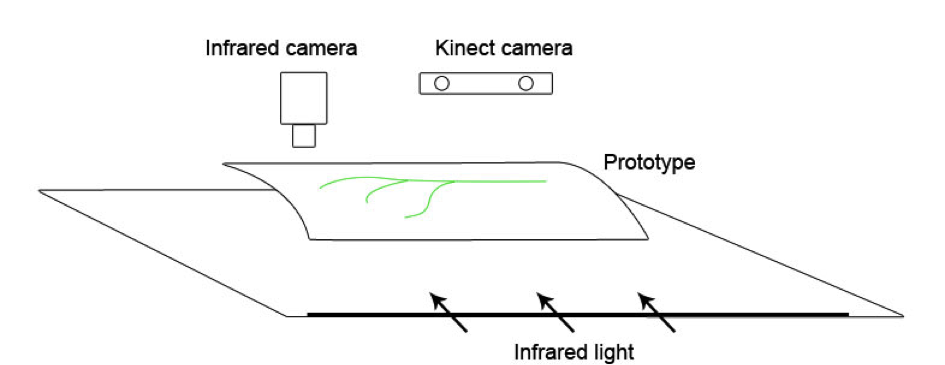
\includegraphics[width=1.0\textwidth]{images/prototype.png}
\label{fig:prototype}
\end{figure}